\chapter{Background}
  The three major goals that we outlined for our initial prototype:
  sharing affect, status, and story, led us to two broader themes.
  \begin{enumerate}
  \item Intimacy and Awareness through Technology.
  \item Catalyzing Support During Crises
  \end{enumerate}

\section{Intimacy and Awareness Through Technology}
  The sharing of statuses led us to the first theme of
  intimacy and awareness through technology.
  Sharing statuses,
  in the form of availability or affective state,
  was really just one example of providing awareness that was valuable to loved ones.
  Technology is used in many different ways for people to maintain
  awareness of people with whom they have relationships,
  in the workplace or at home,
  and there are correspondingly many opportunities for design.

  \subsection{Designing for Awareness and Expressivity}
    In a survey in 2012, Hassenzhal did a broad survey of published research
    that is related to using technology to mediate intimacy
    \cite{hassenzhal12}
    They found that the hundred of published works in this domain indicate a
    huge interest in designing technology that bring people separated by distance together.
    Of the six broad strategies that Hassenzhal found
    that researchers have used in the past few years to design for intimacy
    (and that they suggest all researchers consider),
    the two most common ones are awareness and expressivity.

    Designing technologies for a multi-person group is unusual because the usual
    standards of usability need to be applied to the unit as a whole, and not just
    the experience of a particular individual. \cite{neustaedter12}
    To better understand intimacy between couples,
    Vetere et al. used cultural probes and interviews in 2005 to find
    common themes that led to several preliminary designs for couples.
    Significant research has also gone into designing for couples that are
    separated by distance,
    a common situation that technology is used to help mediate.
    \cite{vetere05}
    Lottridge et al. designed MissU, which took in data collected from several separated couples
    to learn exactly, what, how, and when they choose to share.
    \cite{lottridge09}
    Octavia et al. studied the relationship between friends separated by distance
    and learned that sharing problems and feelings are crucial to
    maintaining a relationship over distance.
    \cite{octavia07}

  \subsection{Awareness Systems}
    The need for awareness is very common in the domestic realm,
    but the depth, frequency, and degree of need for this awareness from specific individuals
    within a personal network vary.
    \cite{neustaedter06}
    Interpersonal awareness systems are one type of technology used to
    help people maintain awareness of each other.
    In 2004, Markopoulos designed and tested an
    awareness system, ASTRA, for families that shared pictures and snippets from a mobile
    device.
    \cite{markopoulos04}
    ASTRA demonstrated measurable affective benefits for the members of
    two families that field tested the technology.

    Another field study by Brush et al. in 2008,
    designed two prototypes, MessyBoard and SPARCS,
    for sharing photos and goals between extended family members.
    \cite{brush08}
    Their study concluded that asynchronous chat and configurable sharing were
    valuable for user sharing,
    considerations that went into the design of InMind as well.

  \subsection{Technology Probe}
    Particularly inspiring to this work is the idea of a technology probe.
    Initially introduced in 2003 by Hutchinson et al,
    technology probes are a type of design probe that has three goals:
    \begin{enumerate}
    \item Understanding needs and desires of users in the real world.
    \item Field testing an engineered product.
    \item Inspiring the design of other technologies.
    \end{enumerate}

    Since then, technology probes and their variants have been used to explore
    new design concepts and their applications. \cite{vetere05, lottridge09}

\section{Support During Crisis}
  The sharing of stories,
  in the context of using them for reflection and sharing serious thoughts,
  led us to a second theme:
  support during crises,
  specifically social support and helping.
  Sharing stories is one of many ways that
  individuals reach out during life crises.
  and only one of many ways they can be helped.
  Individuals dealing with other major life events or transitions
  reach out to loved ones with many variations of serious stories,
  and helpful responses can take many different forms.

  \subsection{Technology and Social Support}
    The most active community developing software for social support is,
    not surprisingly, in the realm of support for chronic diseases.

    One of the earliest work related to using technology to encourage social
    support was from Morris et al. in 2004,
    who were concerned about the narrowing of social support that faced
    elders coping with cognitive decline.
    Morris et al. emphasized the importance of using technology
    as catalysts for human relationships.
    \cite{morris04}

    In 2010, Skeels et. al used a participatory design methodology to explore what is most useful
    to breast cancer patients.
    \cite{skeels10}
    The support of intimate family relations is a powerful
    resource that could
    have a very positive influence on the experience of individuals going through
    tough transitions.
    With breast cancer survivors and their friends, Skeels et al. compiled a model for how
    suggestions and requests for help can be compiled and managed by patients \ref{fig:skeels_diagram},
    and collected all the many barriers to social support that are common for breast cancer patients.
    The prototype technology they implemented was a website, supported by Facebook Connect,
    that allowed patients to perform those request/help idea management tasks.

      % Homescreen Figure
      \begin{figure}
      \caption{\textbf{System for Soliciting Help} --
      From Skeels et al in 2010. Diagram of proposed method of handling suggestions for ways
      to help breast cancer patients.
      }
      \centering
      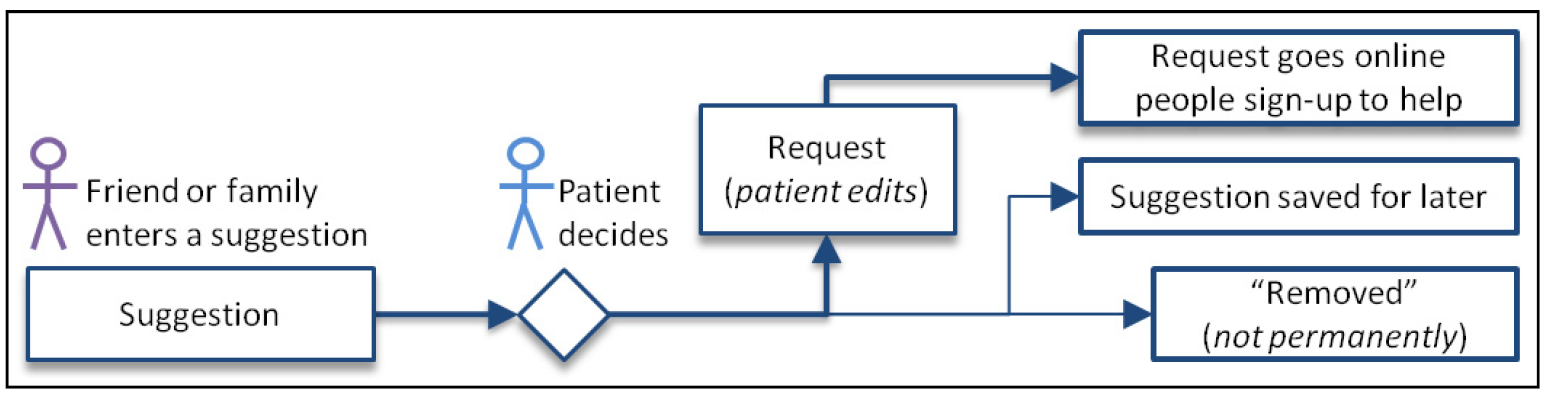
\includegraphics[width=0.80\textwidth]{skeels.png}
      \label{fig:skeels_diagram}
      \end{figure}

    Luxton et al. performed a survey of the many mobile applications available
    to smartphone users in 2011 and
    highlighted many of the health and clinical uses of mobile phones.
    They emphasize that social support is often targeted in clinical practice because
    it can encourage engagement and connection,
    which for many conditions, has positive effects for mental health and well being.
    \cite{luxton11}
